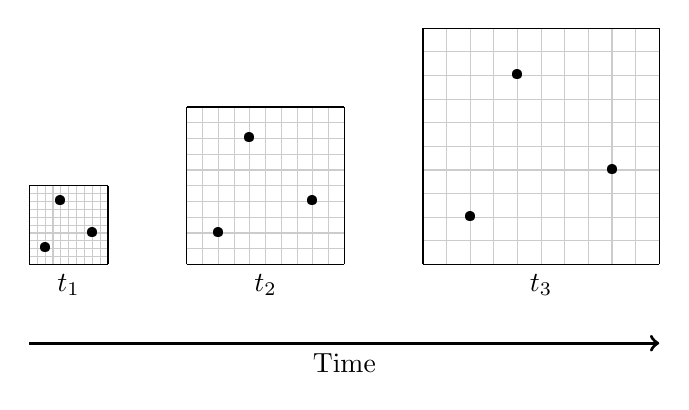
\begin{tikzpicture}
  % Draw the grids
  \draw[step=0.1,opacity=0.2] (0,0) grid (1,1);
  \draw[step=1] (0,0) grid (1,1);

  \draw[xshift=2cm,scale=2,step=0.1,opacity=0.2] (0,0) grid (1,1);
  \draw[xshift=2cm,scale=2,step=1] (0,0) grid (1,1);

  \draw[xshift=5cm,scale=3,step=0.1,opacity=0.2] (0,0) grid (1,1);
  \draw[xshift=5cm,scale=3,step=1] (0,0) grid (1,1);

  % Arrow of time
  \path[->, very thick] 
  (0,-1) 
  edge node[below] {Time}
  (8,-1);

  % Time Labels
  \node[below] at (0.5,0) {$t_1$};
  \node[below] at (3,0) {$t_2$};
  \node[below] at (6.5,0) {$t_3$};

  \def\xa{0.2} \def\ya{0.2}
  \def\xb{0.8} \def\yb{0.4}
  \def\xc{0.4} \def\yc{0.8}
  \def\object{\textbullet}

  \node[] (a1) at (\xa,\ya) {\object};
  \node[] (b1) at (\xb,\yb) {\object};
  \node[] (c1) at (\xc,\yc) {\object};

  \node[] (a2) at ({\xa*2 + 2},{\ya*2}) {\object};
  \node[] (b2) at ({\xb*2 + 2},{\yb*2}) {\object};
  \node[] (c2) at ({\xc*2 + 2},{\yc*2}) {\object};

  \node[] (a3) at ({\xa*3 + 5},{\ya*3}) {\object};
  \node[] (b3) at ({\xb*3 + 5},{\yb*3}) {\object};
  \node[] (c3) at ({\xc*3 + 5},{\yc*3}) {\object};


\end{tikzpicture}
